% 图 C.3 电子绕核运动的两种参考系（两幅转动方向按物理自洽统一为逆时针；
% 原书上幅中心的核符号误印为负号，此处更正为正）
\documentclass[tikz,border=5pt]{standalone}
\usetikzlibrary{arrows.meta}
\usepackage{amsmath}
\usepackage{bm}
\usepackage{fontspec}
\setmainfont{Times New Roman}
\begin{document}
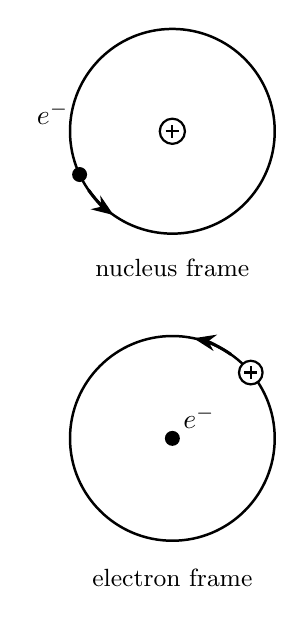
\begin{tikzpicture}[line width=0.8pt,>=Stealth]
% ---------- nucleus frame ----------
\draw[line width=0.9pt] (0,1.75) circle (1.30);
% nucleus at centre
\draw[line width=0.8pt,fill=white] (0,1.75) circle (0.16);
\draw[line width=0.8pt] (-0.085,1.75) -- (0.085,1.75);
\draw[line width=0.8pt] (0,1.665) -- (0,1.835);
% electron on the orbit, moving anticlockwise
\fill ([shift={(0,1.75)}]205:1.30) circle (0.095);
\node at (-1.52,1.98) {$e^-$};
\draw[line width=1.1pt,->] ([shift={(0,1.75)}]215:1.30)
  arc[start angle=215,end angle=235,radius=1.30];
\node at (0,0.02) {\small nucleus frame};
% ---------- electron frame ----------
\draw[line width=0.9pt] (0,-2.15) circle (1.30);
% electron fixed at centre
\fill (0,-2.15) circle (0.095);
\node at (0.34,-1.88) {$e^-$};
% nucleus on the orbit, same sense of rotation (anticlockwise)
\draw[line width=0.8pt,fill=white] ([shift={(0,-2.15)}]40:1.30) circle (0.15);
\draw[line width=0.8pt] ([shift={(0,-2.15)}]40:1.30) ++(-0.08,0) -- ++(0.16,0);
\draw[line width=0.8pt] ([shift={(0,-2.15)}]40:1.30) ++(0,-0.08) -- ++(0,0.16);
\draw[line width=1.1pt,->] ([shift={(0,-2.15)}]55:1.30)
  arc[start angle=55,end angle=78,radius=1.30];
\node at (0,-3.92) {\small electron frame};
\end{tikzpicture}
\end{document}
